% !TEX root =./paper.tex

% Set the title of the paper
\newcommand{\papertitle}{Preliminary Experimental Evaluation of Automated Language-Independent Code Smell Detector}

% Include details of the authors 


% The paper may need to be submitted as "double-blind",
% in which case, none of the authors should be revealed.
% If this is the case, uncomment the line below.
% (This command may also be used elsewhere in the paper,
% e.g., acknowledgements.)
% See also \ifnotdoubleblind command in commands.tex
%
%\newcommand{\doubleblind}{[Details suppressed for double-blind review.]}

% The authors of the paper.
% Add in your name, and any collaborators as needed.
%
\newcommand{\firstauthor}{Yanqiao Chen}
\newcommand{\firstauthoraffiliation}{Allegheny College}
\newcommand{\firstauthorcountry}{China}

%\newcommand{\collaboratorone}{Collaborator 1}
%\newcommand{\collaboratoroneaffiliation}{Collaborator University}
%\newcommand{\collaboratoronecountry}{Collaborator Country}

%\newcommand{\collaboratortwo}{Collaborator 2}
%\newcommand{\collaboratortwoaffiliation}{Collaborator University}
%\newcommand{\collaboratortwocountry}{Collaborator Country}

%\newcommand{\collaboratorthree}{Collaborator 3}
%\newcommand{\collaboratorthreeaffiliation}{Collaborator University}
%\newcommand{\collaboratorthreecountry}{Collaborator Country}

\newcommand{\lastauthor}{Gregory M. Kapfhammer}
\newcommand{\lastauthoraffiliation}{Allegheny College}
\newcommand{\lastauthorcountry}{USA}


% Set the format of the paper.
% Different formats are possible, ensure only one is selected:
%
% \input{formats/acm/conference}
%\input{formats/acm/manuscript}
\input{formats/ieee/conference}
%\input{formats/plain/plain}
%\input{formats/plain/plain-no-date}
%\input{formats/springer/lncs}


% Include packages and key macros. Add to contents of these files as required by
% your paper.
% Packages used by the paper

\usepackage{booktabs}
\usepackage{graphicx}
\usepackage{xspace}
\usepackage{dblfloatfix}
\usepackage{amsmath}
\usepackage{array}
\usepackage{xcolor} % for row colors
\usepackage{colortbl} % for color in tables
\usepackage{cellspace}
\usepackage{nicematrix}
\usepackage{mbpx}

\input{commands}
\input{constants}
% Words and phrases that need to be spelt
% and formatted consistently

\newcommand{\etc}{etc.\xspace}
\newcommand{\etal}{et~al.\xspace}
\newcommand{\ie}{i.e.\xspace}

\newcommand{\GitHubLink}{https://github.com/TreeNose/TreeNose}


\begin{document}

% Include the abstract and perform formatting tasks as dictated by the style
\preabstract
\begin{abstract}

A code smell is a code-design issue that can lead to decrease
in code quality, thereby hindering developers from reading or maintaining
a software program. Code smell detection tools help developers by
automatically checking the existence of code smells. Code smell detection
tools have the potential to be language-independent, because common code
smells occur in many different programming languages.
A language-independent code smell detector can set unified detection rules
across programming languages, which is especially useful in multi-language
software development. However, few code smell detection tools support multiple
programming languages. To fill the aforementioned gap, this paper presents a
tool, called \texttt{TreeNose}, for detecting code smells across programming languages.
\texttt{TreeNose} can detect 5 types of code smells across multiple languages
(i.e., Python, Java, and JavaScript) and its extensible design enables it
to support additional languages. This paper answers three research questions
to explore the quality of \texttt{TreeNose} and structural patterns of code smells
in different languages. In order to answer those questions, we evaluated
\texttt{TreeNose} on 16 open-source projects implemented
in the three chosen programming languages and the combinations of those languages, comparing
its results to those arising from the use of traditional language-specific
code smell detectors in an manual annotation study. 
As a result, \texttt{TreeNose} has a
F1 score of 0.94 for the selected code smells in the chosen systems.
The experimental results also revealed that Complex Conditional code smell counts for a significant amount
in all language systems with high percentages from 32\% to 51\%. 
It also showed that Long Method code smell with 38\% is common in JavaScript, and Long Class code smell with 30\% is common in Java.
Finally, the results showed that every single-language system has certain code smells 100\% more common than the other languages,
which indicates that programming languages have strong tendencies to have specific code smells.
\end{abstract}

\postabstract

% Sections of the document. These are some typical ones. Add and remove these as
% needed.
%
% NOTE: file names should always be lower-cased. This helps for cross-OS
% compatibility. Separate words with hyphens. In other words, use "kebab-case":
% https://wiki.c2.com/?KebabCase
%
\section{Introduction}~\label{sec:introduction}

\vspace*{-1em}

% Code smells are important
% Manual checking is error-prone
% Automated tools are needed

Code smells are a series of code-design-related concerns that may decrease
readability \cite{5741260,SANTOS2018450} and maintainability
\cite{6392174,6405287} of software projects, ultimately limiting opportunities
for future maintenance \cite{Fowler_Beck}. Even though developers acknowledge
the negative influence of code smells on project quality~\cite{developersCare},
manual smell detection remains a error-prone and resource-consuming process
\cite{DetectingDefectsInObject}. To automate this process, different code smell
detection tools rely on detection methods like abstract syntax tree (AST)
analysis~\cite{Lenarduzzi2023}, textual analysis~\cite{Palomba}, or machine
learning~\cite{ML}. Developers also use popular, yet language-specific, smell
detection tools (e.g., PMD~\cite{PMD} and CheckStyle~\cite{CheckStyle}) in the
continuous integration setup of projects like Apache Commons
Lang~\cite{ApacheCommonsLang} and Jenkins~\cite{Jekins}.

% Multi-language projects are common
% Code smell detection is not commonly language-independent
% Maintaining multiple tools is a cumbersome task

One of the characteristics of many modern software projects is their use of
multiple programming languages \cite{723183}. The combination of programming
languages allows developers to mix and match the functionalities and libraries
that are best supported by specific programming language \cite{7476675}.
However, the complexity of multi-language software projects increases the
difficulty of project comprehension and maintenance \cite{7476675,
10.1109/SCAM.2012.11, 7396422}. Along with the complexity, these multi-language
software projects also introduce the pressing challenge of code smell detection.
Most of the existing code smell detection tools are designed to detect code
smells in a single programming language. Multi-language projects, like Jenkins
\cite{Jekins}, use more than one detection tool, thereby introducing the
burdensome need to consistently configure multiple smell detection tools.

% There are benefits to having a language-independent smell
% detection tool, but sadly one does really not exist yet!
% This is the pain that we solve in the next paragraph!

While a limited number of code smell detection tools are language-independent,
most code smells are. For example, Long Method, one of the most prevalent code
smells \cite{developersCare}, can exist in many programming languages. Due to
the language-independence of code smells, code smell detection tools also have
the potential to be language-independent. For instance, Van Emden and Moonen,
the creators of an early code smell detection tool, indicated that their
detection approach in Java had the potential to be applied to other programming
languages in the future \cite{1173068}. Furthermore, Abidi~\etal{} built a
multi-language design smells (i.e., anti-patterns and code smells) detection
tool to detect 15 multi-language-specific design smells for programs that
combine Java and C/C++ \cite{MultiLanguageCodeSmells,Fault-Prone}. A truly
language-independent smell detection tool would offer a unified detection
experience for use in both multi-language software projects and across many
single-language projects.

% Describe TreeNose tool and its features,
% making sure to mention that it is language-independent
% and that it is highly extensible due to Treesitter

Addressing this need, this paper presents a language-independent code smell
detection tool, called \texttt{TreeNose}, to detect 5 types of code smells ---
Complex Conditional, Long Class, Long Method, Long Message Chain, Long Parameter
List --- across multiple programming languages. \texttt{TreeNose} leverages
Treesitter \cite{treeSitter}, a general-purpose parser generator, to parse the
source code of multiple programming languages into an AST. Leveraging the
generated AST, \texttt{TreeNose} queries the nodes with detection rules to
detect targeted code smells with configurable thresholds. Since it builds on
Treesitter, \texttt{TreeNose} is highly extensible, allowing developers to add
new programming languages without rewriting its source code and to support new
smells with minimal engineering effort.

% Design of the experiments

We experimentally evaluated \texttt{TreeNose} on 9 open-source projects
implemented in Java, JavaScript, or Python, comparing the performance of
\texttt{TreeNose} with the combination of 3 language-specific code smell
detection tools in a manual annotation study. Augmenting the 9 projects with 7
new ones, we also investigated the characteristics of code smells in different
programming languages.
%
% Overview of the experimental results
%
The results showed that \texttt{TreeNose} achieved a precision of 92\% and an F1
score of 0.94 in detecting code smells in the chosen programming languages. We
also found that (i) Complex Conditional accounts for 42\% of the total code
smells detected on average, making it the most common smell in the selected
programming languages; (ii) programming languages have strong tendencies towards
specific smells, such as JavaScript containing 3 times more Long Method smells
than the other languages; (iii) multi-language projects have more evenly
distributed code smells than single-language ones.
%
% Listing of the key contributions
%
The contributions of this paper are:

\begin{enumerate}
    %
    \item A language-independent code smell detector that finds 5 types of code
        smells across programming languages.
        %
    \item An experimental evaluation of \texttt{TreeNose} to study its accuracy
        for multiple programming languages.
        %
    \item An investigation of the prevalence and distribution of code
        smells in different programming languages.
        %
\end{enumerate}

\vspace*{-0.5em}

\section{Background and Related Work}~\label{sec:background}

\vspace*{-1em}

% Explain the basics of code smells and their importance and prevalence

{\bf Code Smells}.
Originating from Fowler and Beck's \textit{Refactoring} book, code smells are
important considerations for both researchers and practitioners.
The research community has defined numerous code
smells~\cite{Pysmell,SQLAntipatterns,CleanCode,RefactoringWorkbook}, with
Jerzyk recently releasing an online catalog with 56 common code
smells~\cite{Jerzyk2023}.
At the same time, researchers investigated the effects of code smells on
maintainability (e.g.,~\cite{6392174, 6405287}) and studied developers' opinion
of code smells~\cite{developersCare}, ultimately identifying what real-world
developers consider the top 15 most common code smells.
Moreover, Tufano~\etal{}~\cite{whenandwhy} and Peters and
Zaidman~\cite{lifespan} characterized the lifespan of code smells in software
projects.
Finally, Santana~\etal{} found that strong agglomerations of certain code
smells often occur in software projects~\cite{Santana} and Pascarella~\etal{}
showed that code reviews significantly reduce the severity of code
smells~\cite{Pascarella}.

% Provide a very brief overview of code smell detection tools.
% Key insight to get across:
% - AST
% - Text
% - Machine Learning
% Real tools called linters

{\bf Code Smell Detection}. Due to their negative influence on software
quality, developers acknowledge the importance of detecting code
smells~\cite{developersCare} --- even though manual code smell detection is
both error-prone and resource-consuming~\cite{DetectingDefectsInObject}.
%
To automate this process, different code smell detection tools analyze either a
program's abstract syntax tree (AST)~\cite{Lenarduzzi2023} or its
text~\cite{Palomba}, or use machine learning~\cite{ML}.
%
Open-source developers have also created many language-specific linters for
smell detection (e.g., PMD~\cite{PMD} and CheckStyle~\cite{CheckStyle}), while
researchers created and evaluated ones like PySmell~\cite{Pysmell}.

% Multi-language code smells:
% - Why they are important
% - They are common
% Existing tools are not as good as they could be,
% especially when compared to TreeNose

{\bf Multi-Language Code Smells}.
%
Since developers mix and match the best features of programming
languages~\cite{7476675}, real-world software is often multiple-language in
nature~\cite{723183}.
%
Although many language-specific smell detectors find similar code
smells~\cite{CheckStyle,DesigniteJava,Jscent,PMD,Pysmell}, they do so with
differing internal representations and defaults, making their use difficult
either across many single-language projects or in any multi-language one.
%
In response, Abidi~\etal{} defined 12 multi-language
smells~\cite{MultiLanguageCodeSmells}, ultimately discovering that they are
both common and a strong negative influence on software quality~\cite{Abidi2}.
%
Using a multi-language detector implemented with \texttt{srcML}, they found
that multi-language smells are prevalent in multi-language systems and have a
strong negative influence on software readability~\cite{Fault-Prone}.
%
Finally, Nagy and Cleve built a smell detector for SQL statements embedded in
Java code~\cite{SQLInJava}, while Saavedra and Ferreira~\cite{Saavedra2023}
created one for projects in several infrastructure definition languages.
%
Unlike \texttt{TreeNose}, the aforementioned tools do not use Treesitter
parsers, thereby making them both less general-purpose and less extensible.

\begin{figure}[t]
    % Figures should be centered in the page/column
    \centering
    %
    \vspace*{-1em}
    %
    % Figure content goes here. This could be a graphic,
    % a TikZ diagram, etc.
    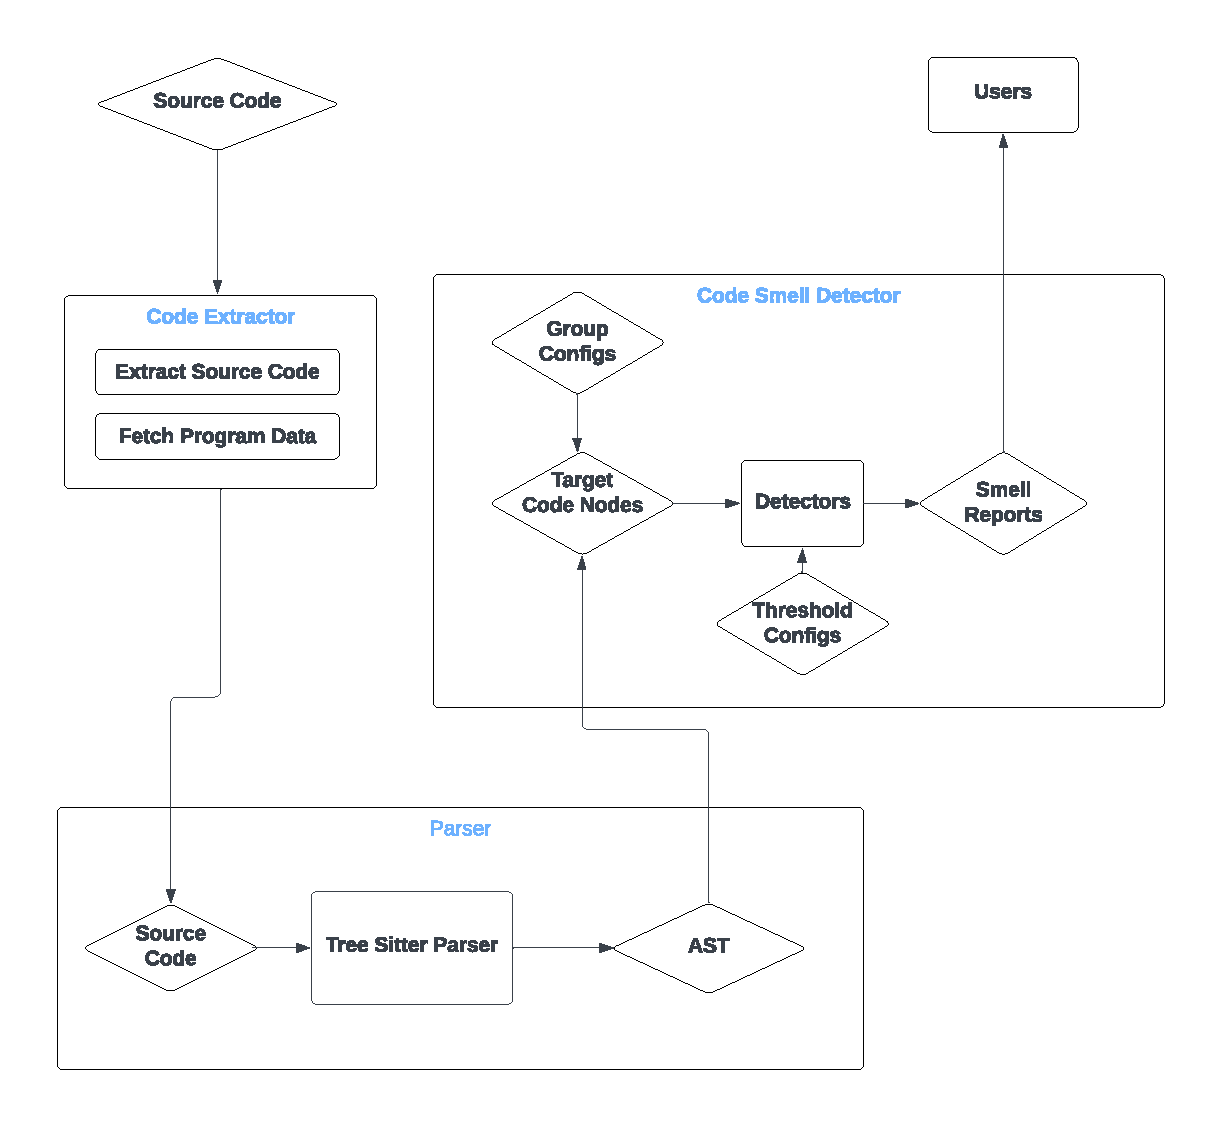
\includegraphics[width=\columnwidth]{graphics/Architecture.pdf}
    %
    \vspace*{-2em}
    %
    \caption{
        % The label should appear _inside_ the caption to ensure
        % Latex numbers it correctly. This is a common gotcha!
        %
        % All figure labels should start with "fig:"
        % So that the figure file can be found easily, the rest of the
        % figure label should be the same as the filename, as it is
        % in this example:
        %
        \label{fig:architecture}
        %
        The TreeNose tool for language-independent code smell detection.
    }
    \vspace*{-1.5em}
    %
    % To save space, you might want to remove space here
    % (use a negative \vspace, e.g. \vspace{-1em})
\end{figure}


% Use tight spacing around the title of the section

\vspace*{-0.5em}

\section{Language-Independent Smell Detection}~\label{sec:approach}

\vspace*{-1em}

% Give the basic definitions of the code smells
% Motivate why we picked these code smells
% Note: only four out of the five code smells that
% developers care about are implemented in TreeNose

{\bf Definitions}. Bearing in mind both the top 15 most common code smells
reported by developers~\cite{developersCare} and those smells commonly detected
by existing tools for Java, JavaScript, and Python, we designed
\texttt{TreeNose} to detect these code smells:

\begin{itemize}[leftmargin=*]
	%
    \item \textbf{Complex Conditional (CC)}~\cite{Fowler_Beck}: occurs when a
        conditional clause contains too many conditions, such as nested {\tt
        if-else} statements, and long {\tt switch-case} statements.
	      %
    \item \textbf{Long Class (LC)}~\cite{Fowler_Beck}: evident when a class
        defines too many (or too lengthy of) properties and/or behaviors.
	      %
    \item \textbf{Long Method (LM)}~\cite{Fowler_Beck}: a method has too many
        lines.
        %
    \item \textbf{Long Message Chain (LMC)}~\cite{Fowler_Beck}: evident when
        there is a long chain of method calls and/or attribute references.
	      %
    \item \textbf{Long Parameter List (LPL)}~\cite{Fowler_Beck}: occurs when a
        method has too many input parameters.
        %
\end{itemize}

{\bf Detection Technique}. \texttt{TreeNose} adopts AST-based approach to detect
code smells. The Fig.~\ref{fig:architecture} discloses the architecture of
\texttt{TreeNose}. \texttt{TreeNose} executes 3 steps to detect target code
smells. 1. Extract source code from the project, 2. Parse the source code to
AST, 3. Analyze AST to detect code smells.

\textbf{Step 1: Extract Source Code}: \texttt{TreeNose} recursively extracts
source code matching with the target programming language from the
project. During this procedure, \texttt{TreeNose} fetches all target files
unless the file or the path is in the ignore list.

\textbf{Step 2: Parse Source Code to AST}: \texttt{TreeNose} parses the source
code to AST with Treesitter \cite{treeSitter}. Treesitter is a parser generator
tool that generates AST in multiple programming languages. It currently
supports 18 language bindings. Treesitter decouples the parser from the
language grammar, making it possible to parse the source code in multiple
programming languages.

\textbf{Step 3: Analyze AST to Detect Code Smells}: \texttt{TreeNose} analyzes
AST to detect code smells. Before the analysis, our developers categorize the
language-specific Treesitter AST nodes like method and function across
programming languages into language-independent groups. This categorization
enables \texttt{TreeNose} to execute the same detection process for nodes in
the same group across multiple programming languages. During the analysis,
\texttt{TreeNose} queries AST and searches for the associated components in
AST. When locating the components, \texttt{TreeNose} calculates the metrics
against the thresholds. Table~\ref{tab:metrics-and-thresholds} shows the
detection metrics with default thresholds for each code smell. Finally,
\texttt{TreeNose} generates reports with the list of code smells detected in
the project.

% Tables should be placed at the top of pages/columns
% where they can.
%
% This can be ensured by using the [t] parameter to the
% "\begin{table}" declaration.
%
\begin{table}[t]
    % Figures should be centered in the page/column
    \centering
    %
    \caption{
        % The label should appear _inside_ the caption to ensure
        % Latex numbers it correctly. This is a common gotcha!
        %
        % All table labels should start with "tab:"
        % So that the figure file can be found easily, the rest of the
        % table's label should be the same as the filename, as it is
        % in this example:
        %
        \label{tab:metrics-and-thresholds}
        %
       Criteria thresholds for identifying smells with TreeNose.
    }
    %
    % Depending on the template, some breathing space might need to
    % be added (use \smallskip \medskip etc.) here
    %
    % Or, to save space, you might want to remove space
    % (use a negative \vspace, e.g. \vspace{-1em})
    %
    %
    % Table content goes here. Use this file to specify the
    % table's column headings. The data should be automatically
    % output from a program processing the raw experimental data
    % and should be inputted from another file. This enables
    % the data to change, if for example, the experiment data
    % needs to be updated.
    %
    % Do not use vertical rules. Ensure you use \toprule, \midrule
    % and \bottomrule from the "booktabs" package effectively.
    %
    % Numbers should be right justified (use "r"),
    % text left justified (use "l").
    %
    % For example:
    %
    \renewcommand{\arraystretch}{1.2}
    \begin{tabular}{@{}lll@{}}
        \toprule
            % use a new line for each column if needed
            {\bf Code Smell}
            &
            {\bf Criteria Threshold}
            &
            {\bf Metrics}
            \\
            %
        \bottomrule
        \input table-data/metrics
    \end{tabular}
    %
    % To save space, you might want to remove space here (use a negative
    % \vspace, e.g. \vspace{-1em})
    \vspace{-1em}
\end{table}


\section{Experimental Evaluation of TreeNose}~\label{sec:evaluation}

\vspace*{-1em}

% Integration of content to save space and be direct!
% 1) Describe the context for the empirical study
% 2) Describe the research questions

\noindent
This paper's experiments answer these research questions:

\begin{itemize}[leftmargin=*]

    % RQ1: Manual annotation study
    %
    \item {\it RQ1: How does \texttt{TreeNose} perform in different languages?}
        To answer RQ1, we evaluated \texttt{TreeNose}'s code smell detection
        effectiveness by applying it to 9 open-source projects with at least
        10,000 lines of code written in Java, JavaScript, or Python, as shown in
        the top half of Table~\ref{tab:subject_table}. Adopting a manual
        annotation methodology, we answer RQ1 by calculating precision, recall,
        and the F1 score for both \texttt{TreeNose} and three popular
        language-specific tools.

    % RQ2: Code smell percentages
    %
    \item {\it RQ2: How do code smells distribute in various languages?} To
        answer RQ2, we augmented the 9 projects used to answer RQ1 with 7 more,
        including 4 projects that are multi-language in nature, as shown in
        Table~\ref{tab:subject_table}. Using \texttt{TreeNose}'s output, we
        calculated the percentage of the reported code smells, across the chosen
        projects for each supported language and for multi-language projects.

    % RQ3: Code smell prevalence
    %
    \item {\it RQ3: How often do code smells occur in various languages?}
        Again using the combined subject set in Table~\ref{tab:subject_table},
        we answer RQ3 by calculating a discrepancy score that contextualizes the
        prevalence of a code smell by programming language.

\end{itemize}

% Introduce the subjects (note, now using the term "projects" instead of "subjects")

{\bf Projects}. To empirically answer these three RQs, we applied
\texttt{TreeNose} to real-world open-source projects that met the following
criteria: (i) have commits on main branch in the last year; (ii) have at least
10 thousand lines of code; (iii) have more than 1,000 stars on GitHub; and (iv)
have an implementation entirely in one of Java, JavaScript, or Python or,
alternatively, a multi-language implementation using one or more of the three
aforementioned languages.
%
To answer RQ1, we picked the 9 projects in the top half of
Table~\ref{tab:subject_table}.
%
It is worth noting that, even though \texttt{TreeNose} supports both Python
versions 2 and 3, PySmell only supports Python version 2, thereby necessitating
that all of the Python-based projects must be implemented in version 2 of
Python.
%
In support of the answer to RQ2 and RQ3, the bottom half of
Table~\ref{tab:subject_table} includes one more project in each of the three
chosen languages and four additional multi-language projects.
%
For each project, we performed smell detection on the source code of both the
program and its test suite because the test code is important for a developer
to comprehend and maintain~\cite{ML}.

\begin{table}[h]
    % Figures should be centered in the page/column
    \centering
    %
    \caption{
        % The label should appear _inside_ the caption to ensure
        % Latex numbers it correctly. This is a common gotcha!
        %
        % All table labels should start with "tab:"
        % So that the figure file can be found easily, the rest of the
        % table's label should be the same as the filename, as it is
        % in this example:
        %
        \label{tab:subject_table}
        %
        CHARACTERISTICS OF SUBJECT SYSTEMS
    }
    %
    % Depending on the template, some breathing space might need to
    % be added (use \smallskip \medskip etc.) here
    %
    % Or, to save space, you might want to remove space
    % (use a negative \vspace, e.g. \vspace{-1em})
    %
    %
    % Table content goes here. Use this file to specify the
    % table's column headings. The data should be automatically
    % output from a program processing the raw experimental data
    % and should be inputted from another file. This enables
    % the data to change, if for example, the experiment data
    % needs to be updated.
    %
    % Do not use vertical rules. Ensure you use \toprule, \midrule
    % and \bottomrule from the "booktabs" package effectively.
    %
    % Numbers should be right justified (use "r"),
    % text left justified (use "l").
    %
    % For example:
    %
    \renewcommand{\arraystretch}{1.2}
    % \rowcolors{2}{gray!25}{white}
    \begin{tabular}{@{}lllrrrrr@{}}
        \toprule
            % use a new line for each column if needed
            {\bf Project}
            &
            {\bf Organization}
            &
            {\bf Language}
            &
            {\bf Version} 
            &
            {\bf Stars} 
            &
            {\bf KLOC}
            \\



        % Now input the data file Note the filename should not have curly
        % brackets, otherwise latex will generate a warning (see
        % https://tex.stackexchange.com/questions/567985/problems-with-inputtable-tex-hline-after-2020-fall-latex-release
        % as to why)
        
        \bottomrule
        \input table-data/subject_data

    \end{tabular}

    %
    % To save space, you might want to remove space here (use a negative
    % \vspace, e.g. \vspace{-1em})
    \vspace{-1em}
\end{table}


{\bf Methodology}. To answer RQ1, we compared \texttt{TreeNose} with 3
language-specific code smell detection tools, namely PySmell~\cite{Pysmell} for
Python, JScent~\cite{Jscent} for JavaScript, and
DesigniteJava~\cite{DesigniteJava} for Java. All 3 code smell detectors are
language-specific, AST-based code smell detection tools that are open-source;
PySmell was shown to achieve 97.7\% precision in a prior study.
%
In this paper's experiment, we compared TreeNose to the combination of the
other tools, aiming to mimic the scenario in which developers use multiple code
smell detectors to identify language-specific code smells across projects that
use different languages.
%
Since the aforementioned detectors support most of the code smells detected by
\texttt{TreeNose}, we applied them to each project in the top half of
Table~\ref{tab:subject_table}. To quantify the performance of \texttt{TreeNose}
and the other tools, we adopted precision and recall, which are defined as
follows:

\begin{equation}
    \textit{Precision} = \frac{\textit{True Positive}}{\textit{True Positive} + \textit{False Positive}}
\end{equation}

\begin{equation}
    \textit{Recall} = \frac{\textit{True Positive}}{\textit{True Positive} + \textit{False Negative}}
\end{equation}

Combining precision and recall, we also calculated the F1 score, the harmonic
mean of precision and recall, defined as:

\begin{equation}
    \textnormal{F1} = 2 * \frac{\textit{Precision} * \textit{Recall}}{\textit{Precision} + \textit{Recall}}
\end{equation}


\begin{table*}[t]
    % Figures should be centered in the page/column
    \centering
    %
    \caption{
        % The label should appear _inside_ the caption to ensure
        % Latex numbers it correctly. This is a common gotcha!
        %
        % All table labels should start with "tab:"
        % So that the figure file can be found easily, the rest of the
        % table's label should be the same as the filename, as it is
        % in this example:
        %
        \label{tab:annotation_table}
        %
        Precision, Recall, and F1 scores for the TreeNose (TN) and the language-specific (LS) detectors.
    }
    %
    % Depending on the template, some breathing space might need to
    % be added (use \smallskip \medskip etc.) here
    %
    % Or, to save space, you might want to remove space
    % (use a negative \vspace, e.g. \vspace{-1em})
    %
    %
    % Table content goes here. Use this file to specify the
    % table's column headings. The data should be automatically
    % output from a program processing the raw experimental data
    % and should be inputted from another file. This enables
    % the data to change, if for example, the experiment data
    % needs to be updated.
    %
    % Do not use vertical rules. Ensure you use \toprule, \midrule
    % and \bottomrule from the "booktabs" package effectively.
    %
    % Numbers should be right justified (use "r"),
    % text left justified (use "l").
    %
    % For example:
    %
    \renewcommand{\arraystretch}{1.2}
    % \rowcolors{2}{gray!25}{white}
    \begin{tabular}{@{}lrrrrrr@{}}
        \toprule
            % use a new line for each column if needed
            {\bf }
            &
            {\bf TN Precision}
            &
            {\bf LS Precision}
            &
            {\bf TN Recall}
            &
            {\bf LS Recall}
            &
            {\bf TN F1}
            &
            {\bf LS F1}
            \\
            %
        \bottomrule
        \input table-data/annotation_data

    \end{tabular}
    %
    %
    % To save space, you might want to remove space here (use a negative
    % \vspace, e.g. \vspace{-1em})
    \vspace{-1em}
\end{table*}


Since, to our best knowledge, there is no annotated code smell dataset for our
unique combination of projects implemented both in the three languages and in a
multi-language fashion, we designed a manual annotation study inspired by the
design of Palomba~\etal's experiment~\cite{Palomba2018}.
%
To answer RQ1, we first applied both \texttt{TreeNose} and the other tools with
their default thresholds to analyze the projects in the top half of
Table~\ref{tab:subject_table}.
%
Facilitating a comparison between the presented tool and the language-specific
smell detectors, we first set \texttt{TreeNose} as the ``baseline'' detector and
randomly sampled 5 code segments for each smell.
%
Next, the authors of this paper independently inspected these flagged code
smells and determined whether, from a developer's perspective, they were valid
not.
%
The authors then discussed their independent classifications until a consensus
emerged as to whether the detected code smells were valid or
not~\cite{Cruzes2011}.
%
We designated a \textit{True Positive} for \texttt{TreeNose} when the authors
and \texttt{TreeNose} classified the randomly selected code as a smell and a
\textit{False Positive} for \texttt{TreeNose} when we did not classify it as a
code smell and yet the presented tool did.
%
When \texttt{TreeNose} was the baseline technique, we designated a \textit{False
Negative} for the language-specific detector when it did not classify the source
code segment as a smell but we did.
%
At this step in the manual annotation study, we calculated the precision for
both \texttt{TreeNose} and the language-specific detector and both recall and
the F1 score for the language-specific detector.

The next step of the manual annotation study set the language-specific tool as
the baseline technique and randomly sampled 5 source code segments that it
claimed were a code smell.
%
Analogous to the prior setup, this configuration enabled us to calculate
precision for both the language-specific smell detector and \texttt{TreeNose}
and to additionally calculate recall and the F1 score for \texttt{TreeNose}.
%
In the absence of an existing data set with confirmed code smell annotations,
this design for the manual annotation study facilitated the indirect comparison
between \texttt{TreeNose} and the other language-specific detectors.
%
Finally, it is important to note that not all code smells detected by
\texttt{TreeNose} are detected by the other tools. For those code smells, we
skipped them in the calculation of the F1 score for \texttt{TreeNose} because
there is no detection results from the other tools, and labeled them as not
detected in the calculation of the F1 score of the other tools. We made this
decision because the other tools ``silently failed'' to detect these code
smells.

% Cut this content:

% With those metrics, we calculated the precision, recall, and
% F1 score of \texttt{TreeNose}. Then, we conducted the same study with the
% samples from \texttt{TreeNose} to calculate the F1 score of the other tools.
% Finally, we utilized the F1 scores of \texttt{TreeNose} and the other tools to
% compare their performances.

% We, furthermore, conducted such a study with 2 internal developers to manually
% verify code smells. Specifically, we built two spreadsheets for the study. One
% for the code smell reports generated by \texttt{TreeNose}, and another for the
% code smell reports generated by the other tools.

% Within the code smell reports
% generated by the other tools, we randomly selected 5 samples out of each code
% smell in each programming language system, and then put those samples in the
% spreadsheet with their related source code and a column for the detection
% decision of \texttt{TreeNose}.

% By this approach, we can compare the decisions between the \texttt{TreeNose}
% and us, where both can potentially agree or disagree with the other detectors.

% Change 20 to 16 to match up with the Table II Remove "up to" 16 to make it
% precise
%
To answer both RQ2 and RQ3, we applied \texttt{TreeNose} to all of the 16
open-source projects in Table~\ref{tab:subject_table}.
%
% The phrase "the combination of the selected languages" is redundant.
%
% combination of them.
%
% Redundant sentence We implemented \texttt{TreeNose} in the projects and
% analyzed the occurrence of each code smell in the projects.
%
Analyzing the code smell reports of \texttt{TreeNose} helped to characterize the
distribution and prevalence of the selected code smells in different programming
languages, and the target languages' tendencies to contain specific code smells.
%
After this step, we calculated the evaluation metrics reported in
Tables~\ref{tab:percentage_table} and~\ref{tab:occurrence_table}.

% RQ2, we calculate the number of each code smell in individual projects
% ($s_{k}$) and divide it by the total number of code smells in that project
% ({$S$}) to calculate the project-level percentage of the code smell. Then we
% the sum of the project-level percentages in the projects in the language, and
% divide it by the number of the projects in the language ($N_r$) to calculate
% the percentage of the code smell in the language ($P_{k}$).

% In the experiment of the RQ2, we calculate the percentage of each code smell
% out of all the selected code smells as follows:

% Specify the purpose of Equation 4 at beginning to reinforce the relationship
% between the equation and the RQ2

We calculated the distribution of each code smell, denoted $P_{s}$, with the
percentage formula given by Equation~\ref{eq:percentage}. To minimize the bias
introduced by the different project sizes (i.e., KLOC in
Table~\ref{tab:subject_table}), the percentage of the code smell in each project
was calculated and then averaged for the projects implemented with that
programming language.
%
We divided the number of each code smell in a project ($m_{k}$) by the number of
all kinds of code smells in that project ({$M_{k}$}), thus calculating the
project-level percentage. We then took the sum of the project-level percentages
and divided it by the number of the projects in the language ($k$) to calculate
$P_{s}$. The results associated with these percentages are shown in
Table~\ref{tab:percentage_table}.

% \vspace{-0.5em}

\begin{equation}
P_{s} = \left( \sum_{1}^{k}\frac{{m_{k}}}{M_{k}} \right) \div {k} \times 100\%
\label{eq:percentage}
\end{equation}

% As for the RQ3, we would like to quantify the prevalence of the code smells as
% the occurrence of the code smells in each 1000 lines of code on average
% ($C_{s}$). To calculate it, we divide the number of each code smell in
% individual projects ($s_{k}$) by the total number of lines in the project
% ($N_{l}$) to calculate the project-level prevalence of the code smell, and
% then take the average of the occurrences in each project. Finally by taking the
% average of the occurrences in the projects in the language, we calculate the
% prevalence of the code smell in the language as follows:

To answer RQ3, we quantified the prevalence of a code smell as the average
occurrence of the code smell in each 1000 lines of code, denoted as $C_{s}$ and
shown in Equation~\ref{eq:prevalence}. To compute this evaluation metric, we
divided the count of a code smell in one project ($m_{k}$) by the total number
of lines in the project ($N_{k}$), thereby giving the project-level occurrence
of the code smell, and then calculate the language-level occurrence score
($C_{s}$) by averaging the project-level occurrences in the projects in the
language and multiplying the result by 1000.

% \vspace{-0.5em}

\begin{equation}
C_{s} = \left( \sum_{1}^{k}{\frac{m_{k}}{N_{k}}} \right) \div k \times 1000
\label{eq:prevalence}
\end{equation}

% With the prevalence score $C_{s}$, we want to quantify how much one language
% outperforms the others. Therefore, we utilized the discrepancy formula to
% calculate the occurrence discrepancy score. We compared the occurrence of one
% language ($C_{s}$) against the same code smell in the combination of the other
% programming languages ($C_{O}$). We calculate the occurrence discrepancy score
% (D) of each code smell in the projects as follows:

Leveraging the code smell occurrence score $C_{s}$ from
Equation~\ref{eq:prevalence}, we calculated the discrepancy formula shown in the
Equation~\ref{eq:discrepancy} to quantify the classification differences between
the selected programming languages and thereby answer RQ3.
%
We calculated the difference with the occurrence of a code smell in one language
($C_{s}$) minus the same code smell in the combination of the other languages
($C_{O}$), and calculated the occurrence discrepancy score (D) by dividing
$C_{O}$. The results associated with these discrepancy scores are shown in
Table~\ref{tab:occurrence_table}.

% \vspace{-1.0em}

\begin{equation}
    D = (C_{O} - C_{s}) \div C_{O}
    \label{eq:discrepancy}
\end{equation}

In the Equation~\ref{eq:discrepancy}, a positive score indicates that the code
smell occurs less frequently in the language than the other languages, while a
negative score indicates that the code smell occurs more frequently in the
language than the other languages.
%
To represent this clearly in Table~\ref{tab:occurrence_table}, we use $\uparrow$
to designate a positive value for this metric and $\downarrow$ for a negative
one.
%
With that said, the discrepancy score has a range of negative infinity to 1,
where 1 means the code smell doesn't occur in the language at all and 0 means
the code smell occurs in the language as frequently as the other languages.

{\bf Threats to Validity}. The definition of code smell, code that is hard to
subjective, which is one of the main concerns in this research.
We noted that various code smell detection tools
utilize different metrics and thresholds to detect the same code smell.
Therefore, the metrics of \texttt{TreeNose} may not be consistent with the
other tools. Similarly, the selection of metrics and thresholds in
\texttt{TreeNose} may not be optimal for detecting selected code smells. To
mitigate the threats, we conducted an annotation study with 2 internal authors to
evaluate the performance of \texttt{TreeNose} in detecting code smells.

% Remove the sentence cuz it's redundant with the end of last paragraph
% """Another threat is related to the annotation study. To evaluate the
% performance of \texttt{TreeNose}, we conducted an annotation study with 2
% developers. """
%
Another threat is related to the annotation study. With the limited number of
developers in the study, the results may not be generalizable to all developers.
We also noted that the amount of subjects and samples are limited in the study.
Though we ensured the subjects are actively used and well-maintained, the
results may still not be generalizable to all software projects in the target
language. We plan to conduct more studies with more developers and subjects in
the future.

% Note: in my view, the third threat is not a threat to validity but a
% limitation, so we may delete it?

% The third threat is related to the limitation of the selected code smell
% detectors. They didn't detect all the selected code smells, and the results may
% be biased by the missing code smells. To mitigate the threats, we plan to
% implement more code smell detectors in the future to compare the performance of
% \texttt{TreeNose} with more detectors.


\begin{table}[h]
    % Figures should be centered in the page/column
    \centering
    %
    \caption{
        % The label should appear _inside_ the caption to ensure
        % Latex numbers it correctly. This is a common gotcha!
        %
        % All table labels should start with "tab:"
        % So that the figure file can be found easily, the rest of the
        % table's label should be the same as the filename, as it is
        % in this example:
        %
        \label{tab:percentage_table}
        %
        PERCENTAGE OF CODE SMELLS IN PROGRAMMING LANGUAGE SYSTEMS
    }
    %
    % Depending on the template, some breathing space might need to
    % be added (use \smallskip \medskip etc.) here
    %
    % Or, to save space, you might want to remove space
    % (use a negative \vspace, e.g. \vspace{-1em})
    %
    %
    % Table content goes here. Use this file to specify the
    % table's column headings. The data should be automatically
    % output from a program processing the raw experimental data
    % and should be inputted from another file. This enables
    % the data to change, if for example, the experiment data
    % needs to be updated.
    %
    % Do not use vertical rules. Ensure you use \toprule, \midrule
    % and \bottomrule from the "booktabs" package effectively.
    %
    % Numbers should be right justified (use "r"),
    % text left justified (use "l").
    %
    % For example:
    %
    \renewcommand{\arraystretch}{1.2}
    % \rowcolors{2}{gray!25}{white}
    \begin{tabular}{@{}lrrrrrr@{}}
        \toprule
            % use a new line for each column if needed
            {\bf }
            &
            {\bf CC} 
            &
            {\bf LC}  
            &
            {\bf LM}
            &
            {\bf LMC}
            &
            {\bf LPL}
            \\



        % Now input the data file Note the filename should not have curly
        % brackets, otherwise latex will generate a warning (see
        % https://tex.stackexchange.com/questions/567985/problems-with-inputtable-tex-hline-after-2020-fall-latex-release
        % as to why)
        
        \bottomrule
        \input table-data/percentage_data

    \end{tabular}

    %
    % To save space, you might want to remove space here (use a negative
    % \vspace, e.g. \vspace{-1em})
    \vspace{-1em}
\end{table}


% Test code may be different than source code of the program

The last threat is due to the decision to include the test code --- along with
the source code of the program under test --- in the analysis used to answer
each research question. While test code is important for developers to
comprehend and maintain in the software development, it may adhere to different
conventions and styles from the program's source
code~\cite{Kapfhammer2004,Kapfhammer2010}. This means that the detection
thresholds of Table~\ref{tab:metrics-and-thresholds}, which are mainly designed
for a program's source code, may not be ideal for the test code. To mitigate
this threat, we plan to conduct future studies that excluding the test code.

% Present the answer to RQ1


\begin{table*}[t]
    % Figures should be centered in the page/column
    \centering
    %
    \caption{
        % The label should appear _inside_ the caption to ensure
        % Latex numbers it correctly. This is a common gotcha!
        %
        % All table labels should start with "tab:"
        % So that the figure file can be found easily, the rest of the
        % table's label should be the same as the filename, as it is
        % in this example:
        %
        \label{tab:occurrence_table}
        %
        DISCREPANCY SCORES OF CODE SMELLS IN PROGRAMMING LANGUAGE SYSTEMS
    }
    %
    % Depending on the template, some breathing space might need to
    % be added (use \smallskip \medskip etc.) here
    %
    % Or, to save space, you might want to remove space
    % (use a negative \vspace, e.g. \vspace{-1em})
    %
    %
    % Table content goes here. Use this file to specify the
    % table's column headings. The data should be automatically
    % output from a program processing the raw experimental data
    % and should be inputted from another file. This enables
    % the data to change, if for example, the experiment data
    % needs to be updated.
    %
    % Do not use vertical rules. Ensure you use \toprule, \midrule
    % and \bottomrule from the "booktabs" package effectively.
    %
    % Numbers should be right justified (use "r"),
    % text left justified (use "l").
    %
    % For example:
    %
    \renewcommand{\arraystretch}{1.2}
    % \rowcolors{2}{gray!25}{white}
    \begin{tabular}{@{}lrrrrrrr@{}}
        \toprule
            % use a new line for each column if needed
            {\bf }
            &
            {\bf CC} 
            &
            {\bf LC}  
            &
            {\bf LM}
            &
            {\bf LMC}
            &
            {\bf LPL}
            \\



        % Now input the data file Note the filename should not have curly
        % brackets, otherwise latex will generate a warning (see
        % https://tex.stackexchange.com/questions/567985/problems-with-inputtable-tex-hline-after-2020-fall-latex-release
        % as to why)
        
        \bottomrule
        \input table-data/occurrence_data

    \end{tabular}

    %
    % To save space, you might want to remove space here (use a negative
    % \vspace, e.g. \vspace{-1em})
    \vspace{-1em}
\end{table*}


{\bf Answering RQ1}. Table~\ref{tab:annotation_table} shows the confusion
matrixes of \texttt{TreeNose} and the other tools in the annotation study. TN
represents \texttt{TreeNose}, and LS represents the other tools. On the
average, \texttt{TreeNose} significantly outperformed the other tools in terms
of precision, recall, and F1 score. With the 0.94 F1 score, we conclude that
\texttt{TreeNose} achieved a high level of accuracy in detecting the code
smells. When there is no value in the table, it means it's not possible to
calculate the recall. For example, \texttt{TreeNose} flagged all the positive
when we selected samples from the \texttt{TreeNose} detection. Therefore, it's
not possible to calculate the recall or the F1 score of \texttt{TreeNose} in
this environment. The same applies to the LS-selected samples. Another
interesting observation is that the LS group achieves 1.0 precision in the
\texttt{TreeNose}-selected samples, but the recall is down to 0.32, which
results in a low F1 score of 0.48. This indicates that the LS group can hardly
detect all the code smells in the \texttt{TreeNose}--selected samples.

{\bf Answering RQ2}. Table~\ref{tab:percentage_table} discloses the percentage
of the code smells in each programming language system. Looking at the table,
we can see Complex Conditional (CC) counts for 46\% of code smells on average,
indicating that it is the most common code smell across programming languages.
the percentage of Long Class (LC) and Long Method (LM) vary significantly in
the Java and JavaScript systems. In the Java system, LC occurs 7 times more
than LM, while in the JavaScript system it's the opposite, LM occurs 30 times
more than LC. This indicates that the programming languages have huge different
tendencies in terms of code smells.

{\bf Answering RQ3}. Table~\ref{tab:occurrence_table} shows the occurrence
discrepancy scores of the code smells in the systems. Since no programming
language contains positive values in every code smell, we conclude no
programming language outperforms the others in every code smell. By looking at
each code smell, we also see programming languages have strong tendencies in
some code smells with at least 1 time worse performance than others. For
example, the Java system has a strong tendency in the Long Class (LC) with 1.24
times worse performance and Long Message Chain (LMC) with 3.56 worse performance than others, 
while the JavaScript system has a strong
tendency in the Long Method (LM) code smell. Python has a strong tendency in
the Long Parameter List (LPL). Multi-Language system, on the other hand, has
weaker tendencies in code smells compared to the other systems with zero
negative values less than - 1.0.

\input{sections/related-work}
\section{Conclusions and Future Work}

% Removed this text and replace it with content that is a little shorter:

% with an annotation study in three programming language system, i.e., Java,
% JavaScript, and Python, and compared it with other language-specific tools in
% a set of high-quality open-source projects in target programming languages.

% As a result, \texttt{TreeNose} achieved a high level of
% accuracy with 0.94 F1 score in detecting selected code smells. As a comparison,
% the combination of other tools achieved 0.48 F1 score. We concluded
% \texttt{TreeNose} is an effective tool for detecting code smells across
% programming language systems. We also analyzed the distribution and prevalence
% of code smells in the programming language systems with \texttt{TreeNose}.

% As results of the analysis, we found that 1. Complex Conditional (CC) is the
% most common code smell across programming languages with 42\% average
% proportion. 2. Programming languages have strong tendencies in some code smells
% with at least 1 time worse performance than others. 3. systems written in
% multi-language have weaker tendencies in code smells compared to the single
% language systems with zero negative values less than - 1.0.

% Review the TreeNose tool, experimental setup, and the results

This paper presents \texttt{TreeNose}, a language-independent code smell
detection tool that leverages Treesitter parsers. \texttt{TreeNose} detects 5
code smells that other language-specific tools (e.g., PySmell and JScent)
commonly support: CC, LC, LM, LMC, and LPL, as defined in
Section~\ref{sec:approach}.
%
Using a manual annotation study, we compared the scores arising from
\texttt{TreeNose}'s classifications to those made with the smell detectors for
Java, JavaScript, and Python,
%
ultimately showing that the language-specific tools yielded an F1 score of 0.48
in comparison to an F1 score of 0.94 from \texttt{TreeNose}.

Building on this compelling result and \texttt{TreeNose}'s capability to
uniformly detect code smells both across projects in different languages
and in multi-language projects, we further used the presented tool to study the
prevalence of code smells.
%
This analysis revealed interesting findings, including the fact that, among the
studied code smells, CC is the most common across the studied projects,
comprising 42\% of the detected smells, including 50\% of those in
multi-language projects.

% Define the future work now that we've shown the tool is so great
% (a) the standard "more of everything"
% (b) highlight that the tool is released
% (c) explain that we want to conduct human studies

Building on these emerging results, we intend to extend \texttt{TreeNose} to
detect more code smells and then evaluate it with both more programming
languages and projects. To extend the manual annotation study, we will engage
additional human annotators to examine more code smells from more projects,
yielding a data set for future studies.
%
Leveraging \texttt{TreeNose}'s open-source release at \texttt{\GitHubLink{}},
we also plan to study how developers use it to detect code smells.


% The paper's bibliography style is set by the paper format.
%
% Ideally, the bibliography itself should be a Git subproject imported into this
% repository.
%
\bibliography{bibtex/bibliography}

\end{document}
